
% TODO: Name all appendices properly in an incremental order!!

% \vspace{-7mm}
% {\let\clearpage\relax
\chapter{Appendix A - Concept Map}
% }
\label{appendix:A-concept-map}
% concept map

\begin{figure}[h!]
\centering
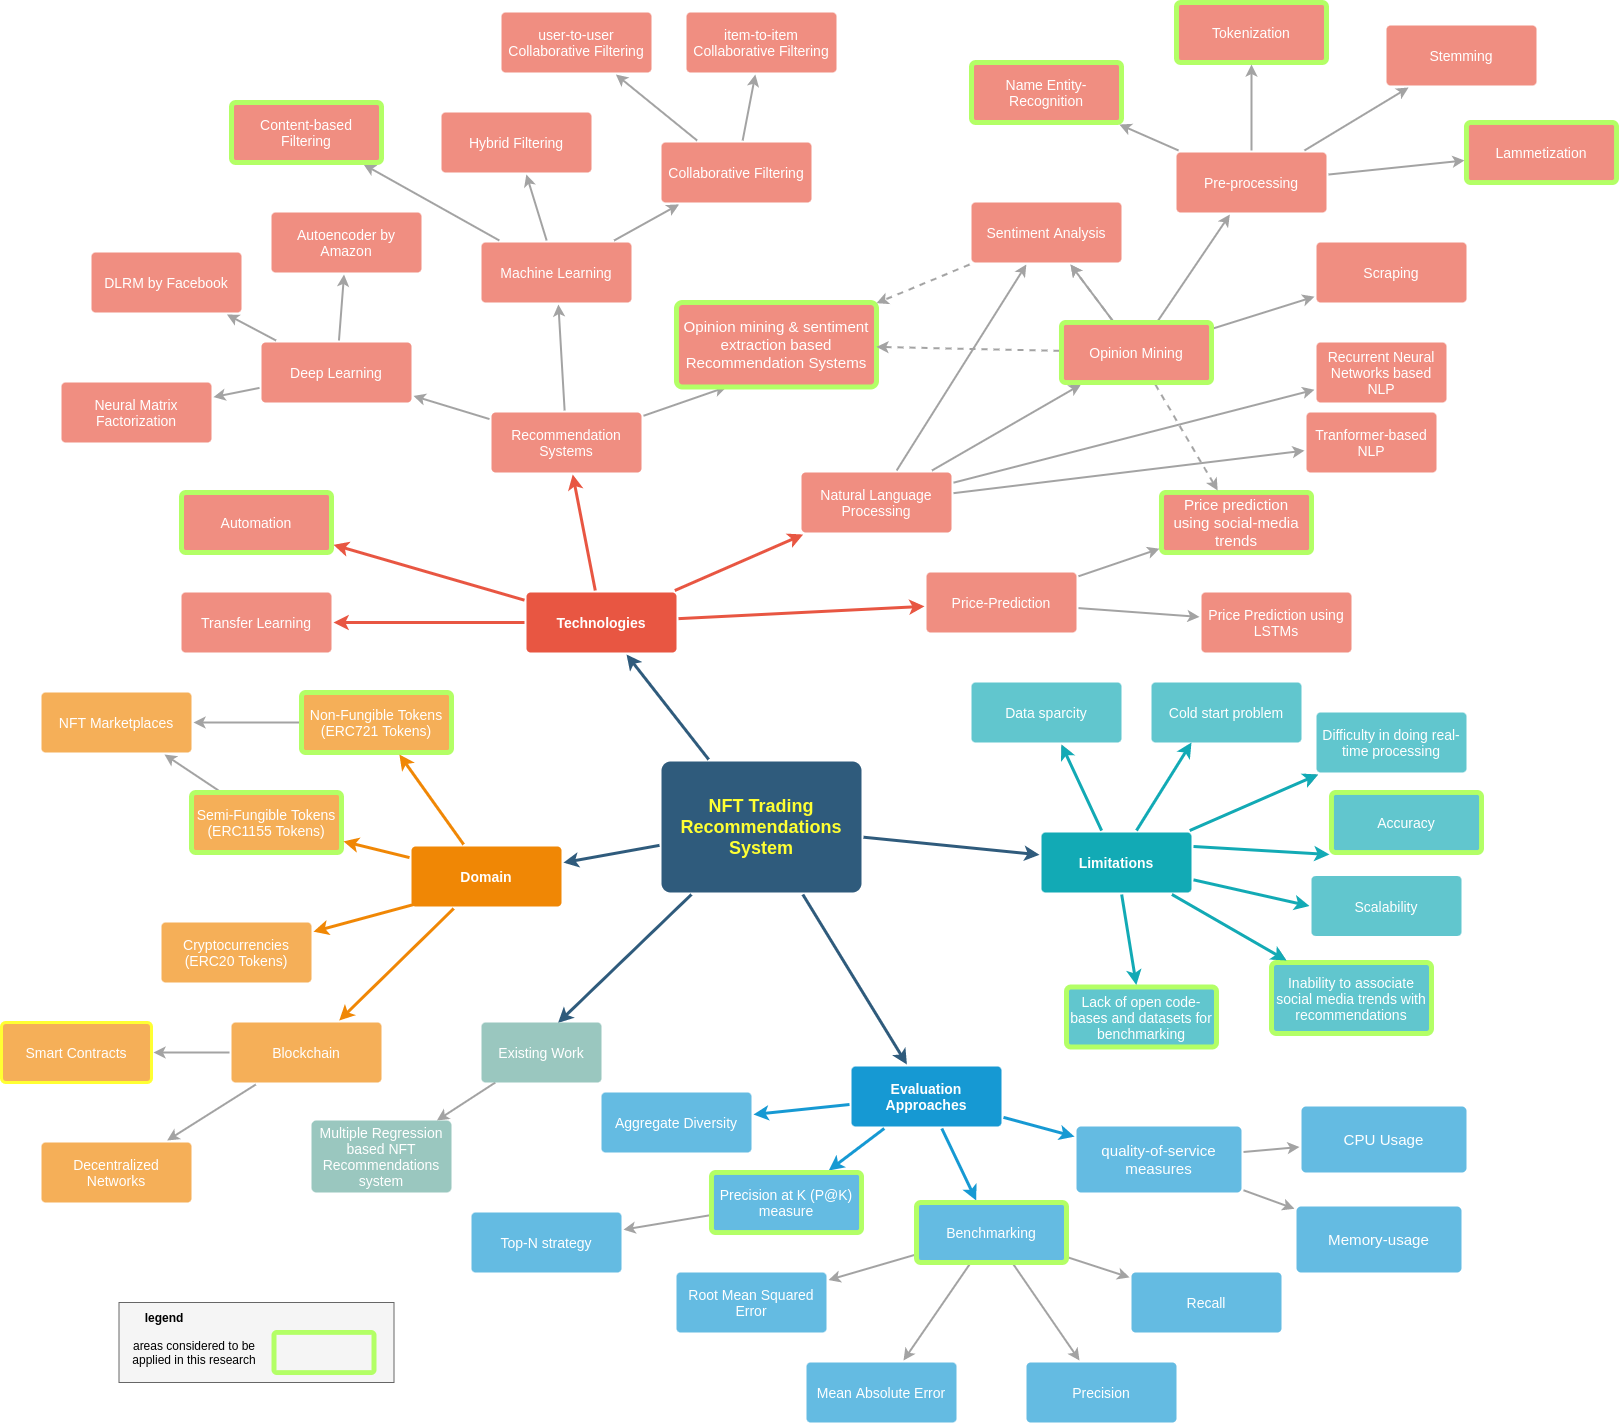
\includegraphics[width=\textwidth]{images/appendix/concept-map.png}
\caption{Concept Map \textit{(self-composed)}}
\label{fig:concept-map}
\end{figure}

% \chapter{Appendix B - Work Breakdown Structure}

% \chapter{Appendix  - Requirement Engineering Survey} (questionnaire)

\chapter{Appendix  - UI Wireframes}
\label{appendix:UI-Wireframes}

\begin{figure}[h!]
\centering
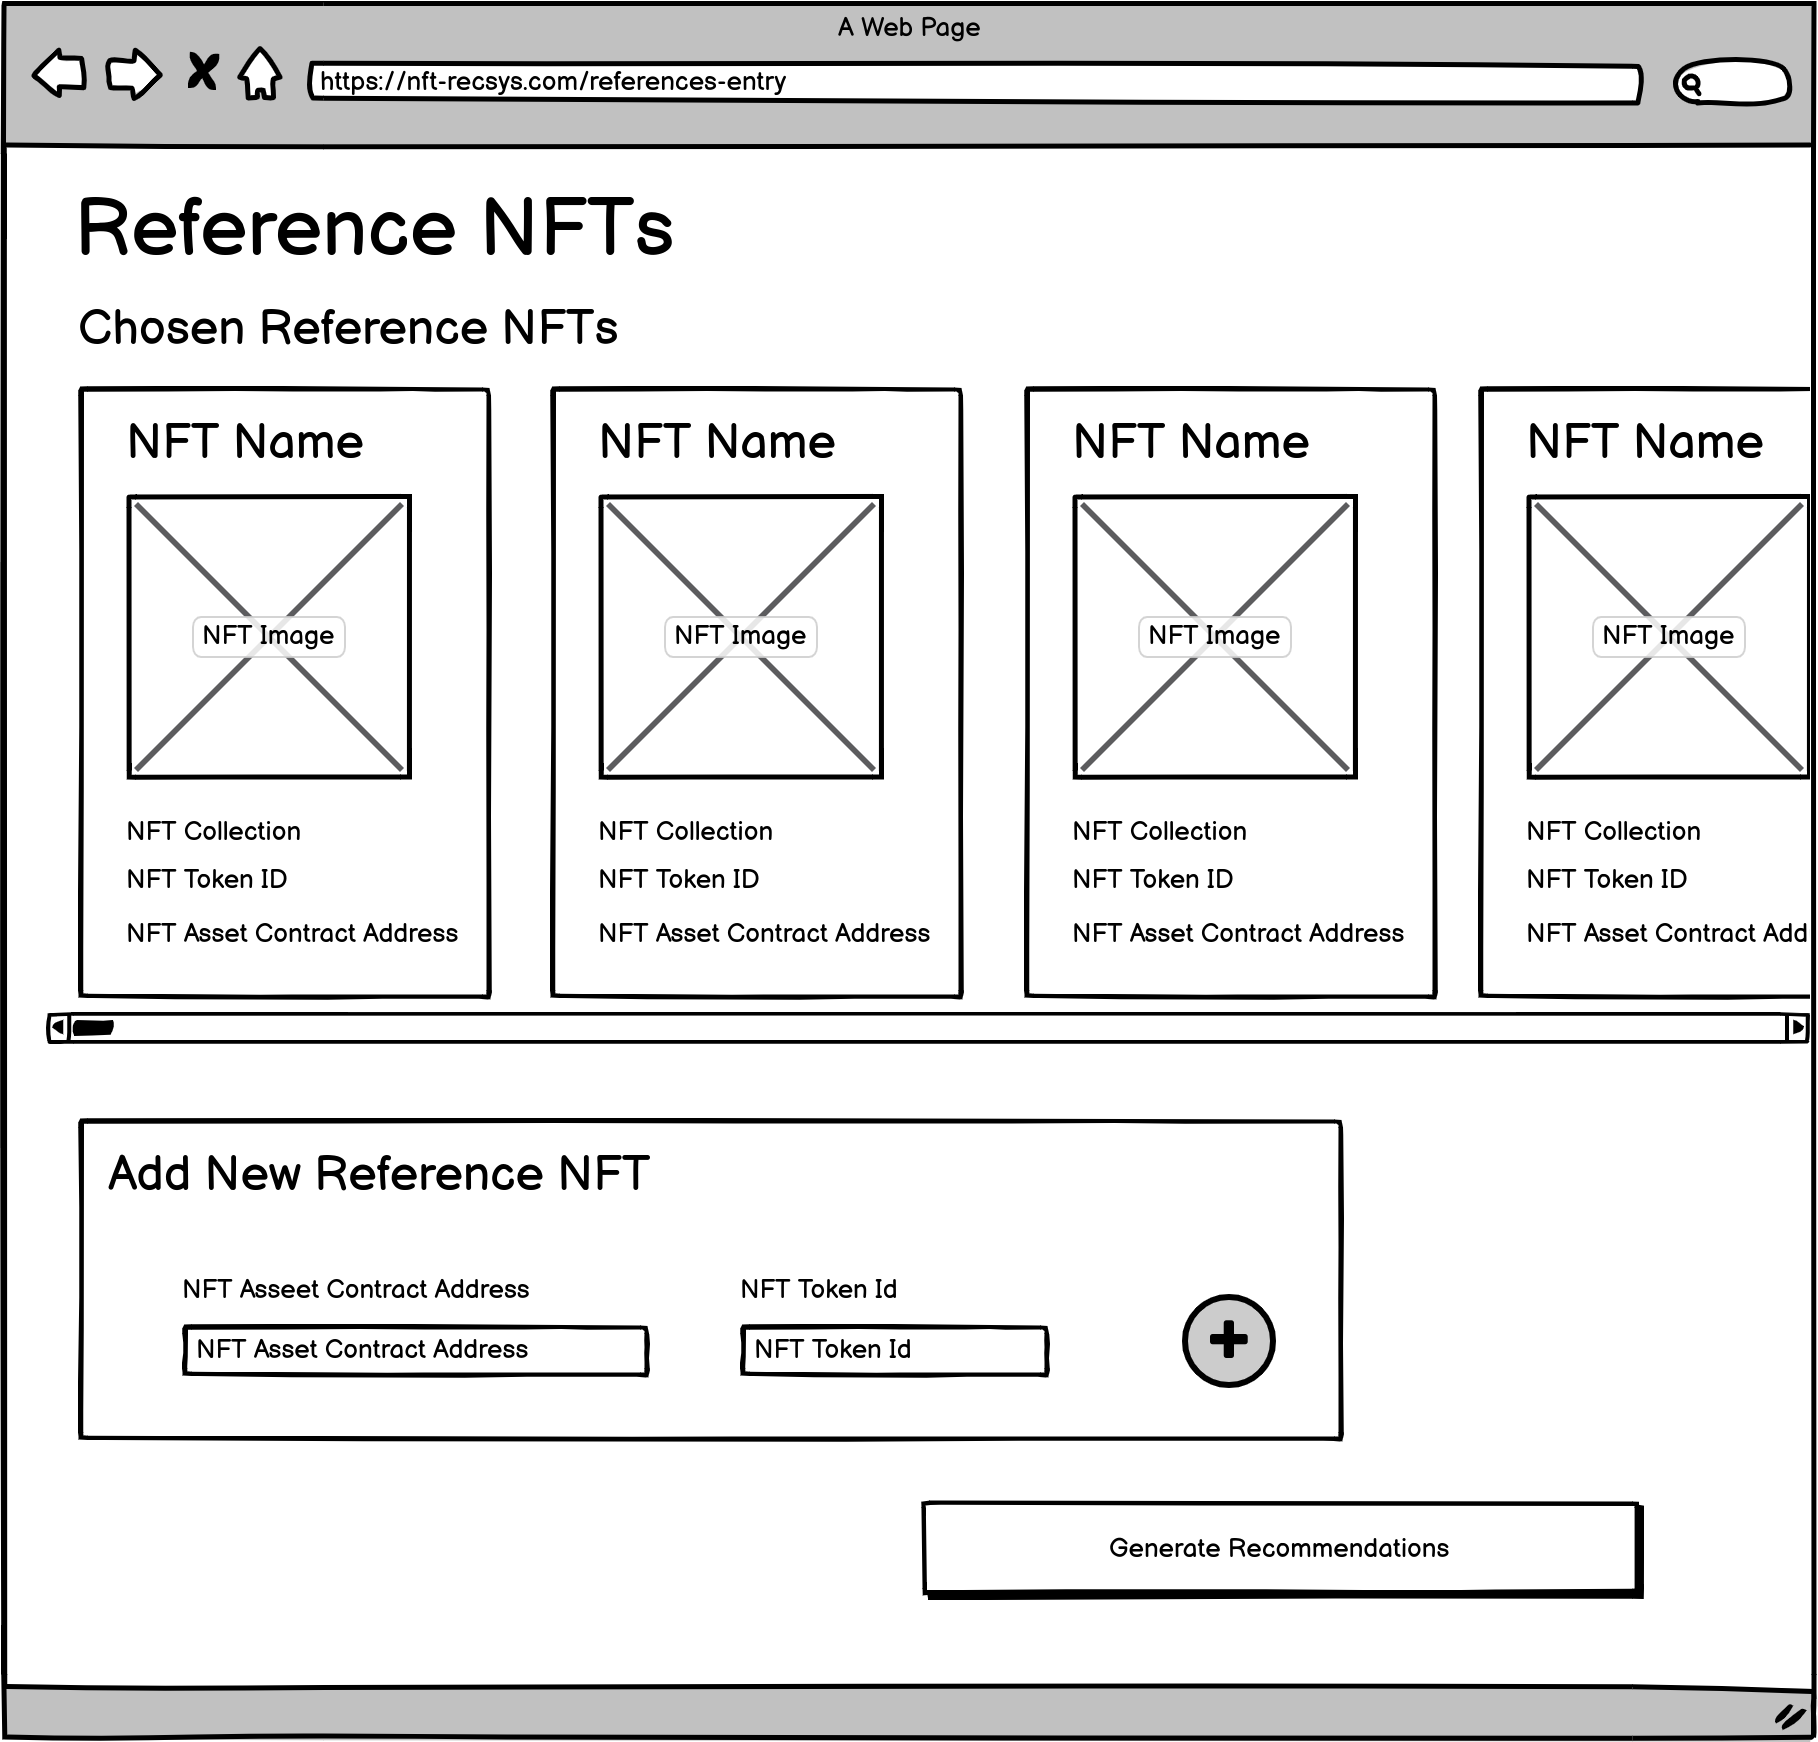
\includegraphics[width=\textwidth]{images/appendix/UI Wireframes/Reference NFT entry.png}
\caption{UI Wireframe - Reference NFT entry \textit{(self-composed)}}
% \label{fig:ui-wireframes-1}
\end{figure}

\begin{figure}[h!]
\centering
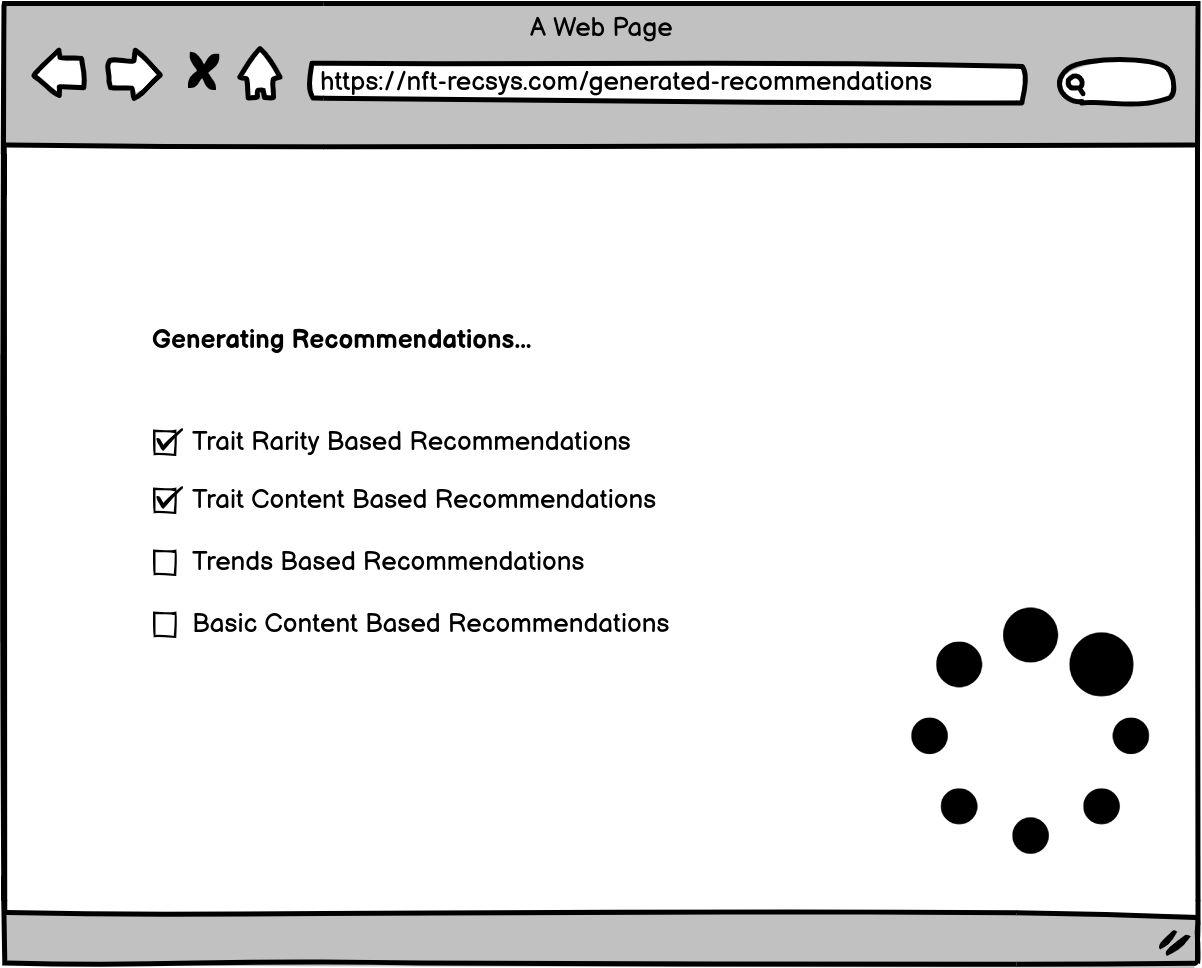
\includegraphics[width=\textwidth]{images/appendix/UI Wireframes/Loading-Generating Recommendations.png}
\caption{UI Wireframe - Loading-Generating Recommendations \textit{(self-composed)}}
% \label{fig:ui-wireframes-1}
\end{figure}

\begin{figure}[h!]
\centering
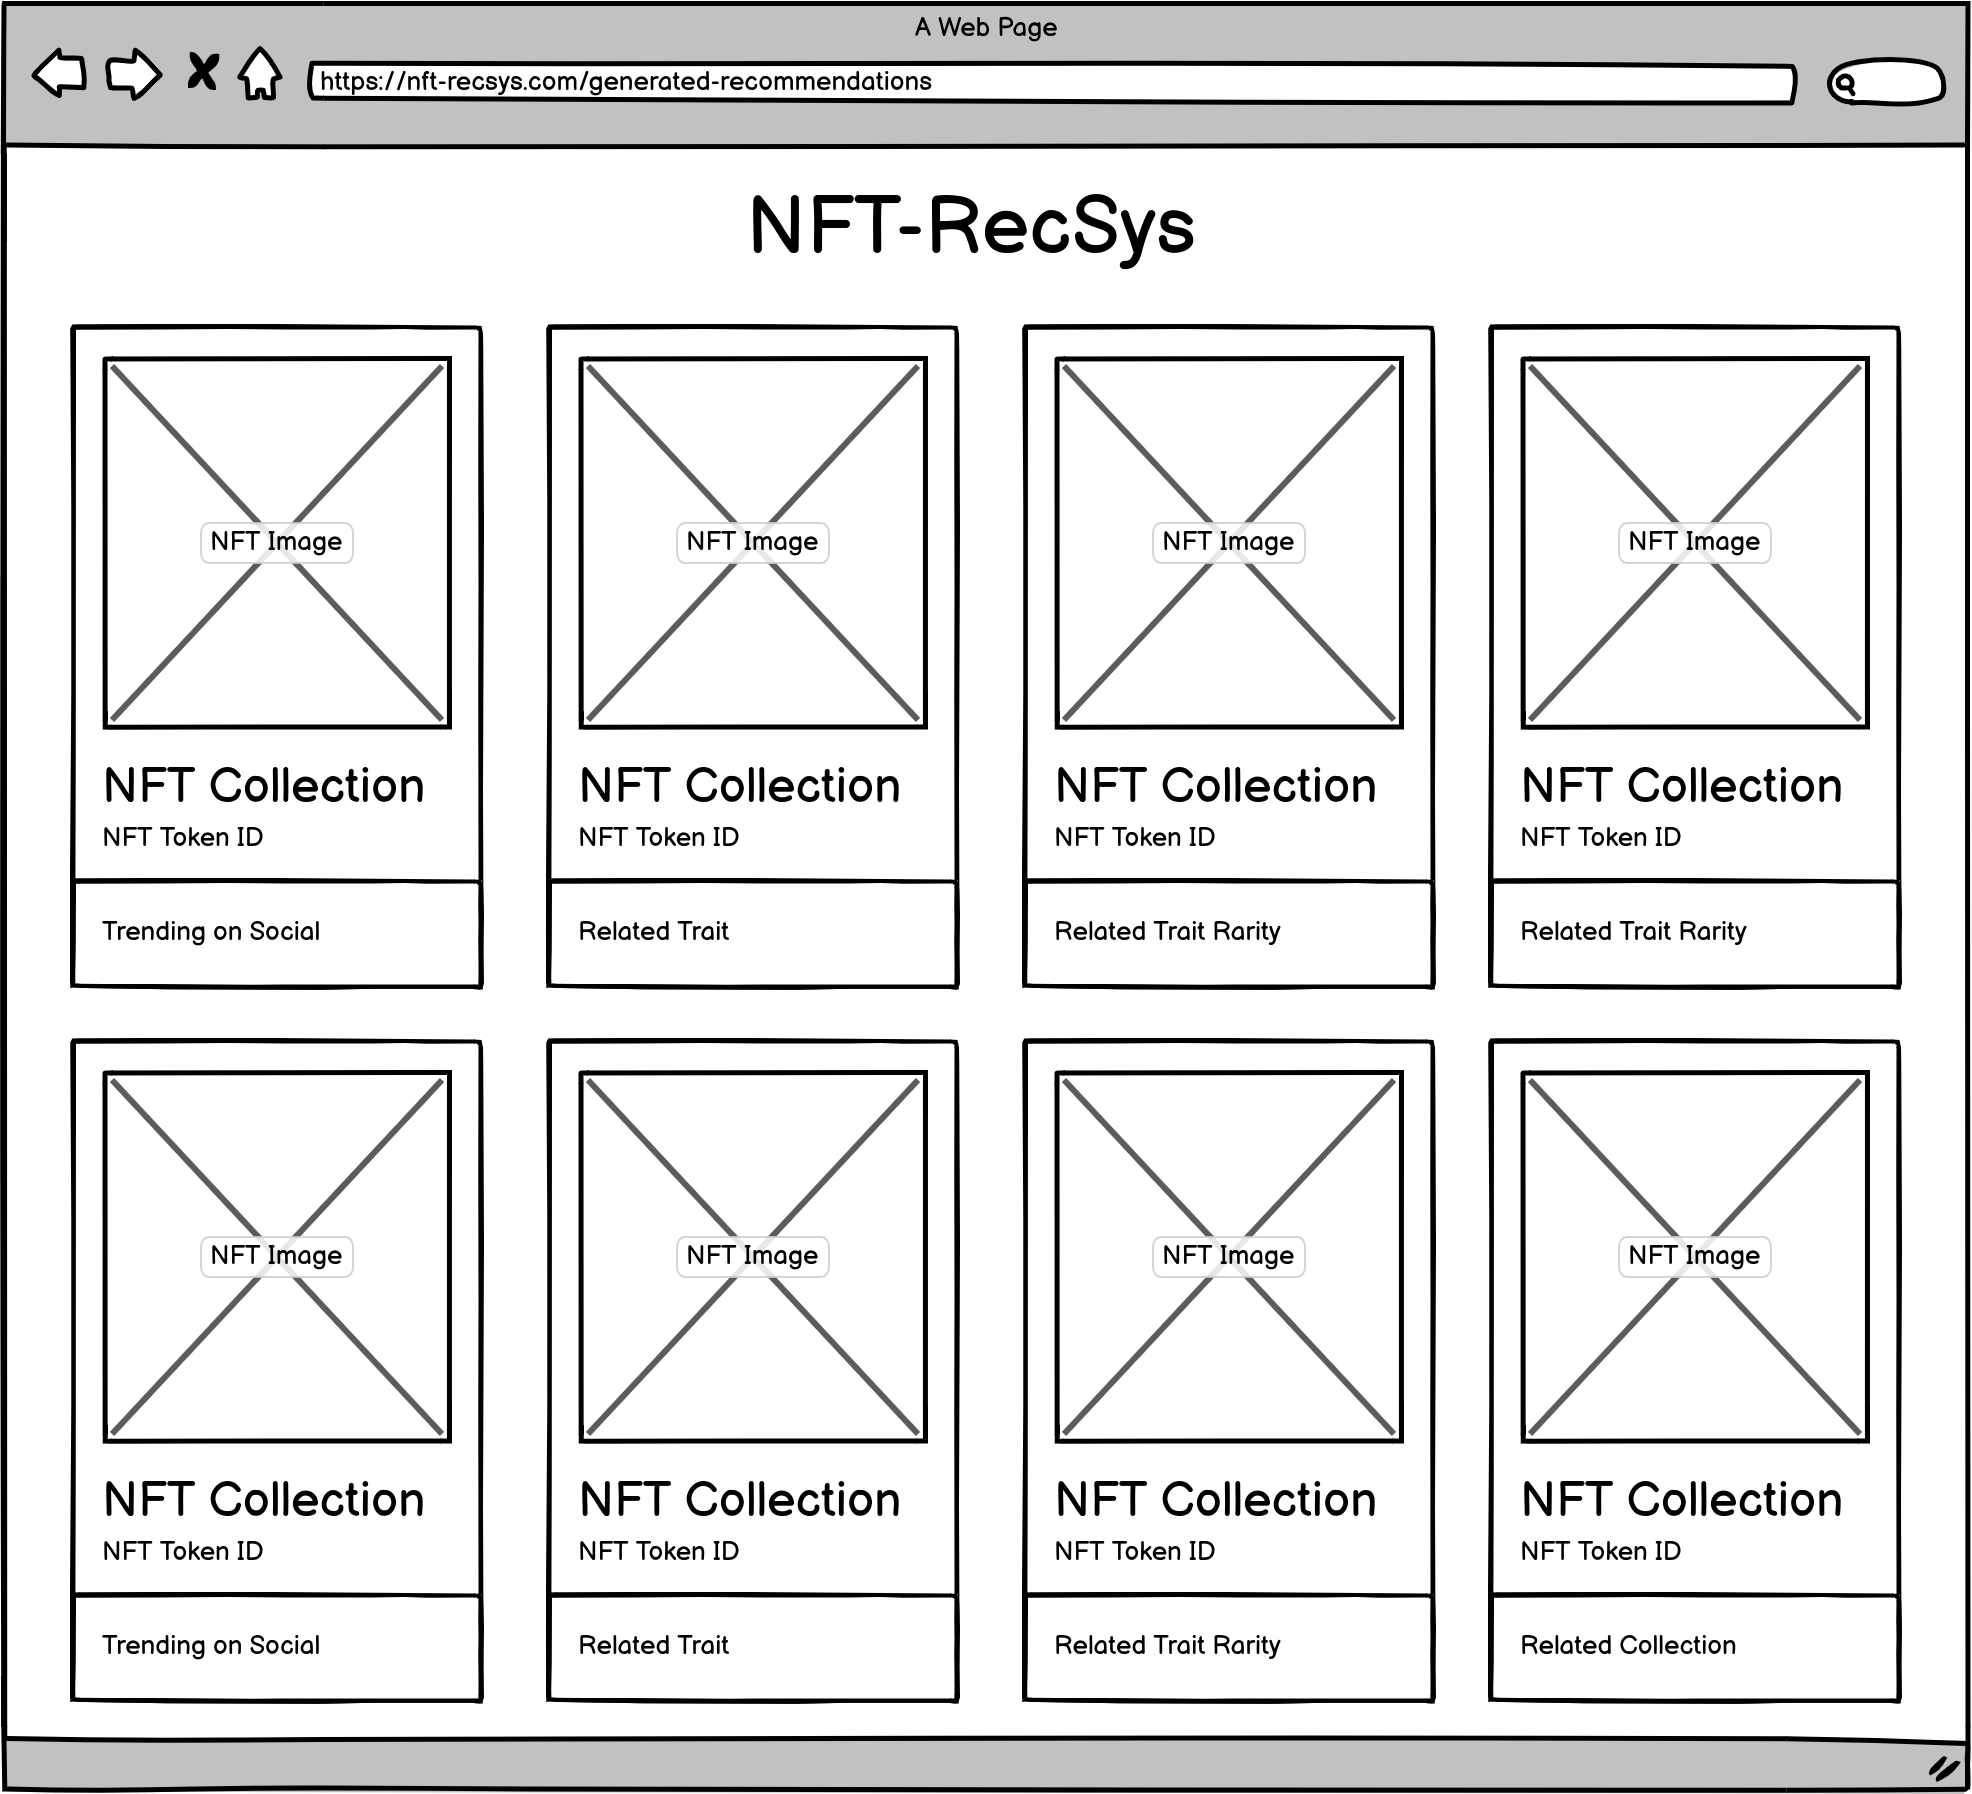
\includegraphics[width=\textwidth]{images/appendix/UI Wireframes/Generated Recommendations.png}
\caption{UI Wireframe - Generated Recommendations \textit{(self-composed)}}
% \label{fig:ui-wireframes-1}
\end{figure}

\begin{figure}[h!]
\centering
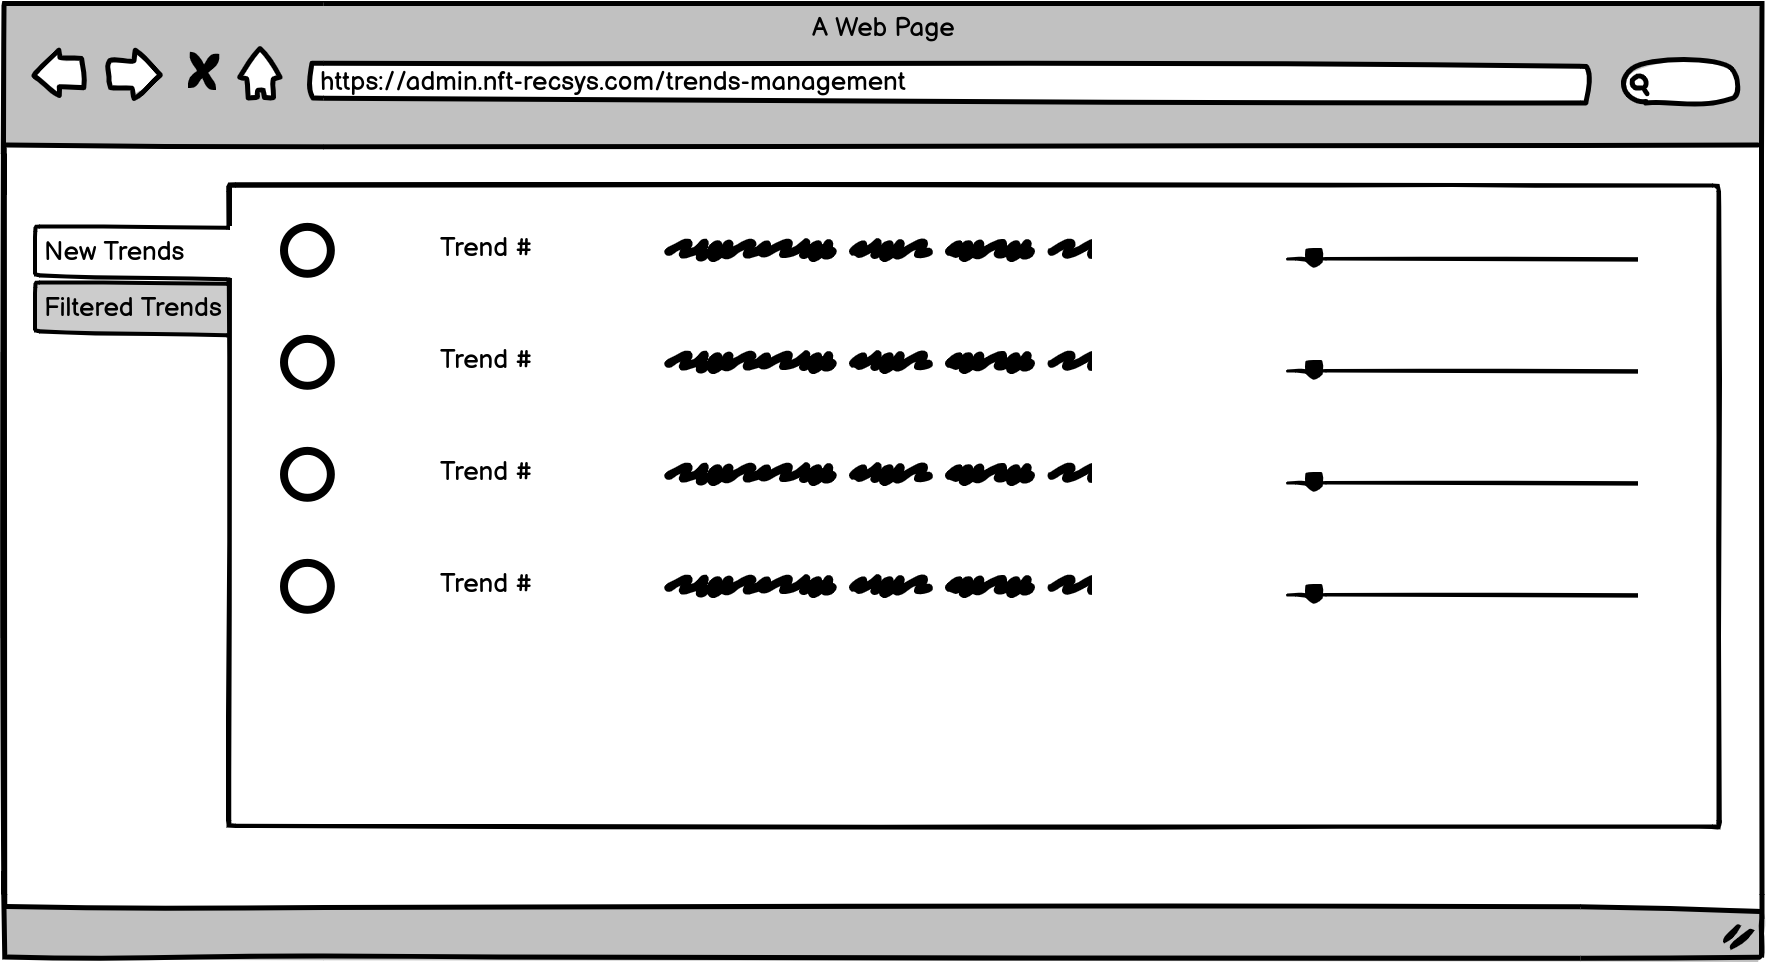
\includegraphics[width=\textwidth]{images/appendix/UI Wireframes/Admin Trends.png}
\caption{UI Wireframe - Admin Trends \textit{(self-composed)}}
% \label{fig:ui-wireframes-1}
\end{figure}

\begin{figure}[h!]
\centering
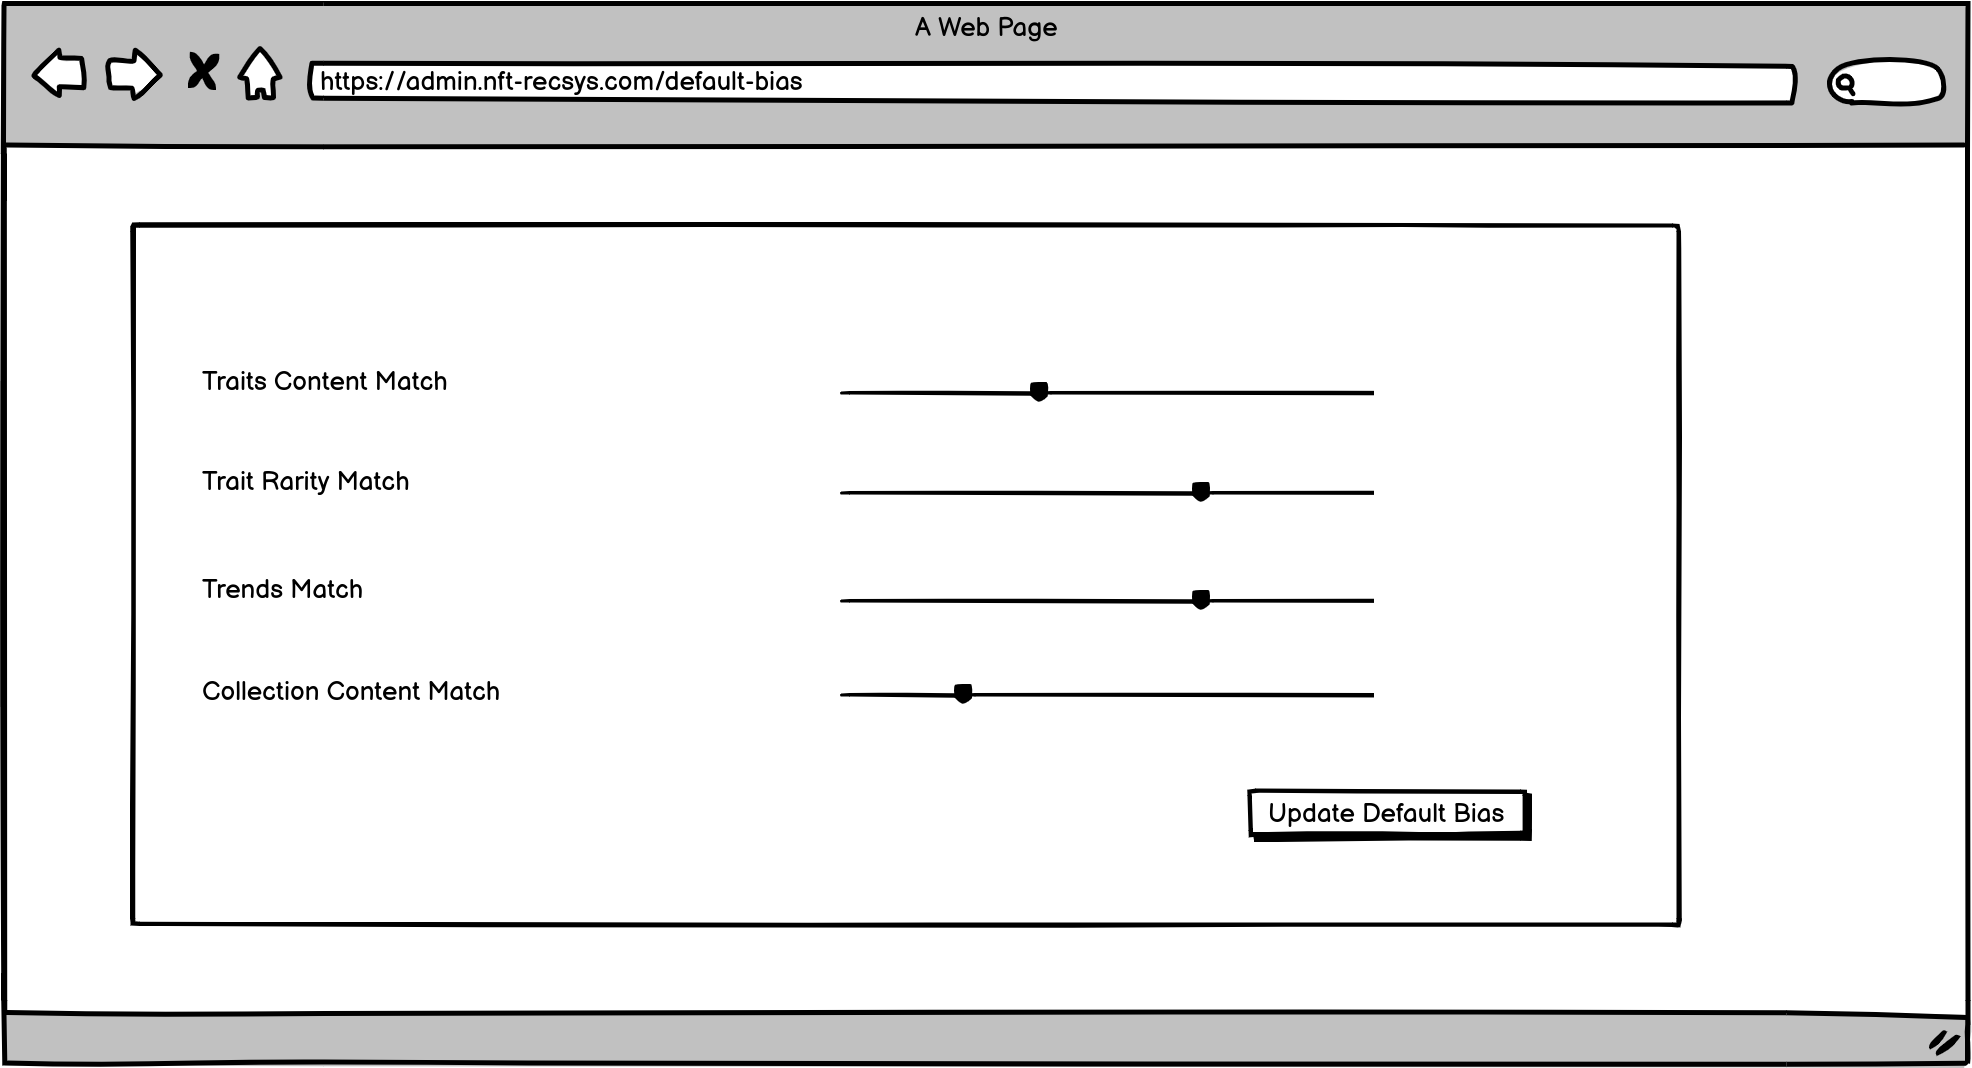
\includegraphics[width=\textwidth]{images/appendix/UI Wireframes/Admin Default Bias selection.png}
\caption{UI Wireframe - Admin Default Bias selection \textit{(self-composed)}}
% \label{fig:ui-wireframes-1}
\end{figure}

\begin{figure}[h!]
\centering
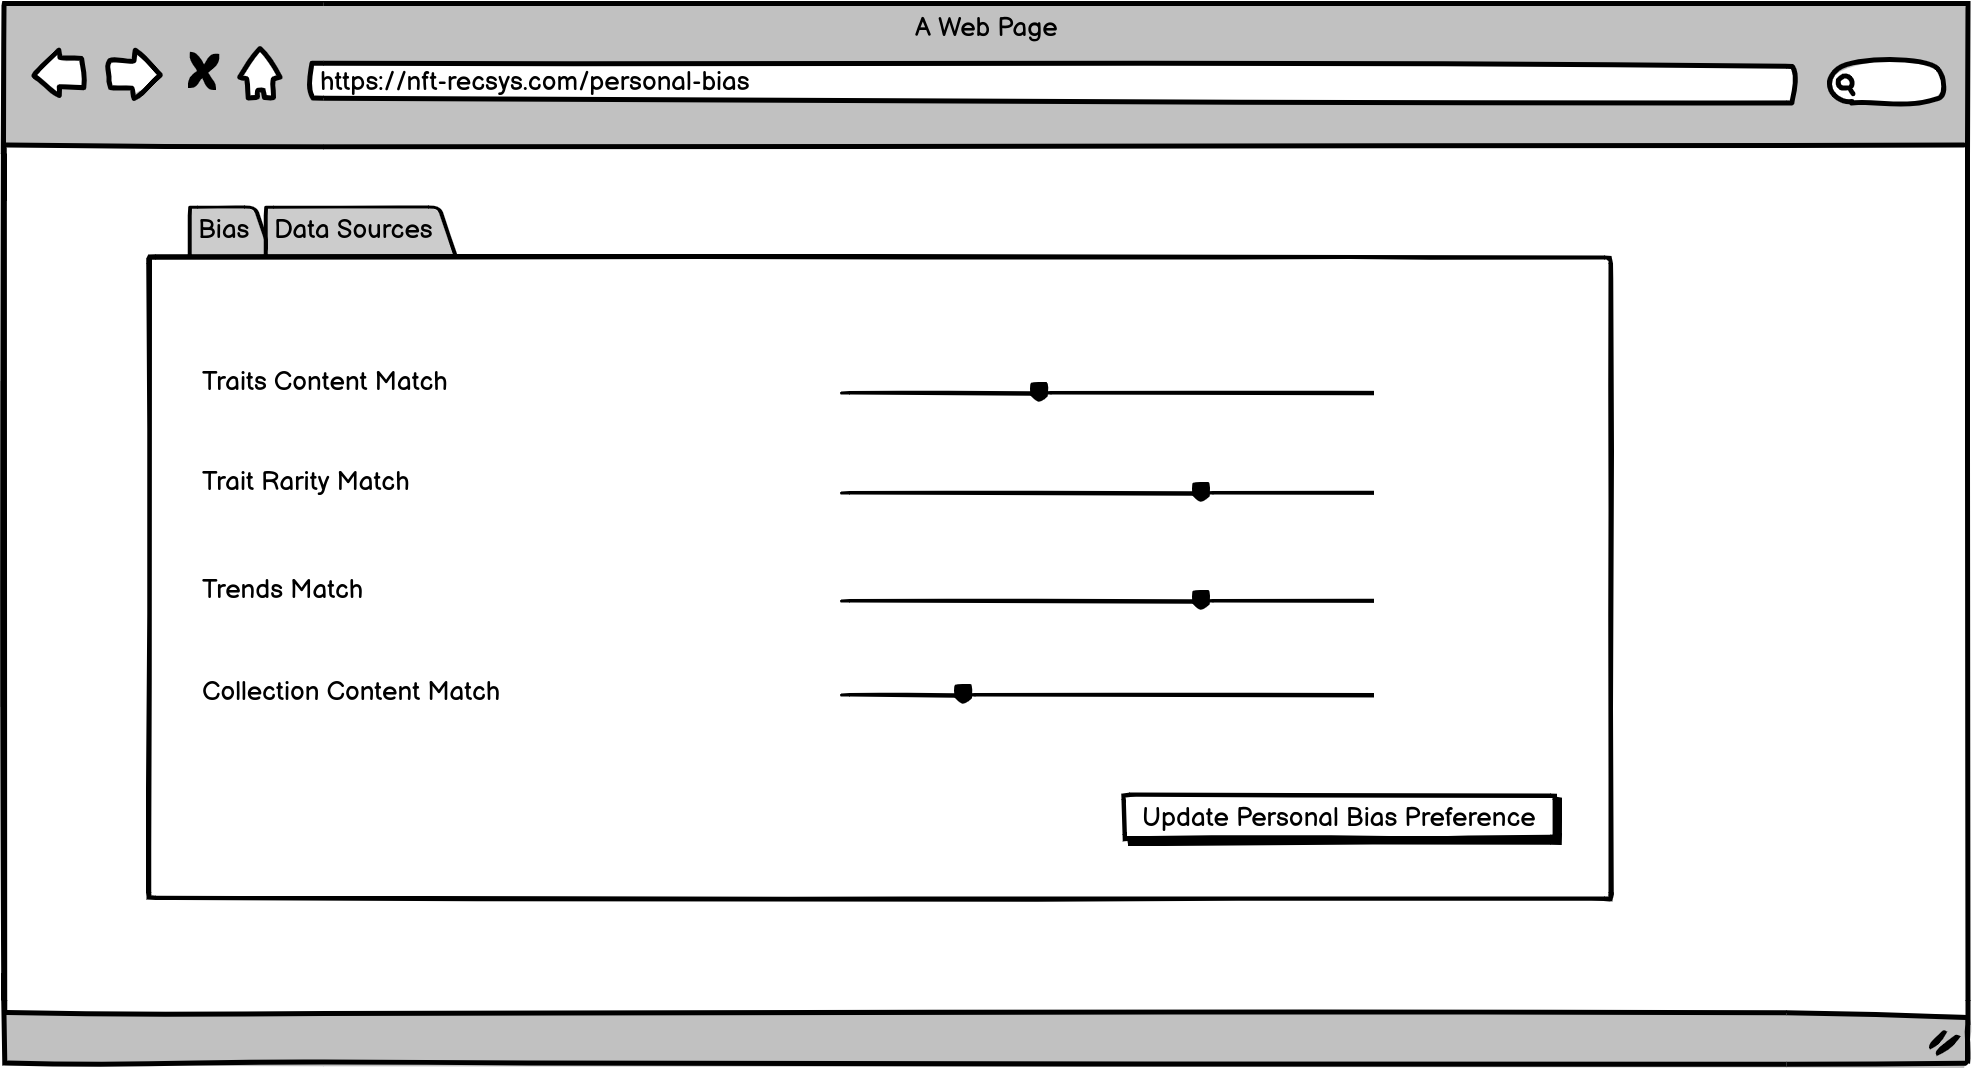
\includegraphics[width=\textwidth]{images/appendix/UI Wireframes/User Bias selection.png}
\caption{UI Wireframe - User Bias selection \textit{(self-composed)}}
% \label{fig:ui-wireframes-1}
\end{figure}


\chapter{Appendix  - Testing}
\label{appendix:testing}

\section*{Appendix 1 - Model Evaluation}

\begin{figure}[h!]
\centering
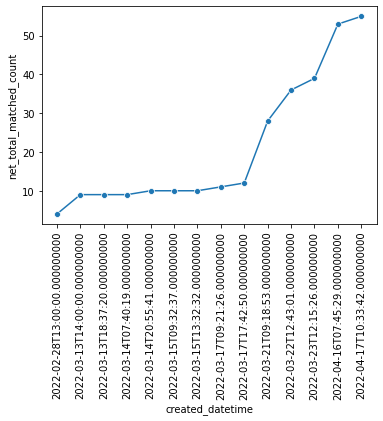
\includegraphics[width=0.6\textwidth]{images/Testing/trends-matches-eval2.png}
\caption{Total Trends based Recommendations made with time \textit{(self-composed)}}
\label{fig:trends-recsys-total-matches}
\end{figure}

\section*{Appendix 2 - Functional Testing}

\vspace{-4mm}
\begin{longtable}{|l|l|p{0.22\linewidth}|p{0.21\linewidth}|p{0.21\linewidth}|l|}
\caption{Testing results of Functional Requirements}
\label{tab:test-func-requirements}
\\ 
\hline
\begin{tabular}[c]{@{}l@{}}\textbf{Test}\\\textbf{Case}\end{tabular}
&
\begin{tabular}[c]{@{}l@{}}\textbf{FR}\\\textbf{ID}\end{tabular}
&
\begin{tabular}[c]{@{}c@{}}\textbf{User}\\\textbf{Action}\end{tabular}
&
\begin{tabular}[c]{@{}c@{}}\textbf{Expected}\\\textbf{Result}\end{tabular} & 
\begin{tabular}[c]{@{}c@{}}\textbf{Actual}\\\textbf{Result}\end{tabular} & \begin{tabular}[c]{@{}c@{}}\textbf{Result}\\\textbf{Status}\end{tabular}
\endfirsthead 
\hline
1 & FR1 & Users adds a chosen \gls{nft} to be considered as the reference & item details are fetched and validated & item details were fetched and validated & Passed \\ 
\hline
2 & FR2 & Admins adds a collection of \gls{nft}s to be used as recommendations. & The details of the \gls{nft}s get fetched and pre-processed for recommendations & The details of the \gls{nft}s were fetched and pre-processed for recommendations & \\ 
\hline
3 & FR3 & A user enters a contract address \& token Id of an \gls{nft}. & The system fetches relevant data of the \gls{nft} & The system fetched relevant data of the \gls{nft} & Passed \\ 
\hline
4 & FR4 & Users sets/ adjusts the bias and parameters to be used & The user specific bias and general bias get adjusted & The user specific bias and general bias were adjusted & \\
\hline
5 & FR5 & Admins adjusts the admin bias & The admin-bias gets adjusted in the system & The admin-bias was adjusted in the system & \\ 
\hline
6 & FR6 & Users clicks a button to generate recommendations & Recommendations are generated and made visible to the user & Recommendations were generated and made visible to the user & Passed \\
\hline
7 & FR7 & A user enters feedback regarding the satisfaction level of the generated recommendations & The feedback of the user is collected and stored in the Database & The feedback of the user was collected and stored in the Database & \\
\hline
8 & FR8 & User requests the reason for recommending the item & Reasons for recommending each item is displayed & Reasons for recommending each item was displayed & Passed \\
\hline
% 9 & FR9 & The system should generate price predictions and consider the results for recommendations. & S & UC5 & \\ 
% \hline
10 & FR10 & User requests featured trending \gls{nft} recommendations & Opinion mining trends data is used to generate \gls{nft} recommendations. & Opinion mining trends data was used to generate \gls{nft} recommendations. & Passed \\
\hline
11 & FR11 & User inputs data-points such as interested public figures, websites to use as opinion mining data for recommendations & The data-points entered are pre-processed and used for trends based recommendations & The data-points entered were pre-processed and used for trends based recommendations & \\ 
\hline
12 & FR12 & Admins inputs data-points such as interested public figures, websites to use as opinion mining data for recommendations. & The data-points entered are pre-processed and used for trends based recommendations & The data-points entered were pre-processed and used for trends based recommendations & \\
\hline
% 13 & FR13 & User-input could be aggregated and used as a reinforcement learning bias for the Recommendations Model. & C & &  \\
% \hline
% 14 & FR14 & The system will not act as a decentralized system. & W & &  \\
% \hline
\end{longtable}

% \section*{Module \& Integration Testing}



\chapter{Appendix C - Evaluations}
\label{appendix:C}

\section*{Appendix C1 - Evaluations received by Evaluators}

% TODO: have a table for each cateogry/ separate by category row.
% OR group evaluators - separate using row with category ID?

\vspace{-4mm}
\begin{longtable}{|p{0.23\linewidth}|p{0.69\linewidth}|}
\caption{Evaluations received by Evaluators}
\label{tab:evaluators-eval-feedback}
\\
\hline
\textbf{Evaluator} & \textbf{Feedback} \endfirsthead
\hline
% name & Qualifications/~ Position of Employment 
\textbf{Mr. Sharmilan Somasundaram}
[\textit{CEO of Niftron - Blockchain as a Service, Certified Blockchain Solution Architect (CBSA)}]
&  Because there's no system like this, it's a good research. The research project is good because gathering data \& domain side is difficult \& new.
The trends based model needs more evaluation. Try synthesizing data to show how recommended items vary across time. Try to show the significance of using the model.
\\
\hline
\textbf{Mr. Nipuna Senanayake} [\textit{}] & The concept of the trends based recommendations system is good. Evaluation of the trends based model is a bit of a concern. Might be possible to evaluate it by web-scraping.
Good amount of work has been done. Keep up the same enthusiasm for research, it will help in the long run, wherever you go.
 \\
\hline
Anonymous [\textit{Blockchain Masters Researcher}] & The research is good, haven't seen \gls{nft} researches that much, although there're quite a lot of Blockchain researches. Will give an A for the project since proper research has been done with the identified research gap.
Price prediction might be possible using art market pricing (if available) since the \gls{nft} market is similar to the market.
\\
\hline
 & \\
\hline
\end{longtable}

\section*{Appendix C2 - Evaluation of Functional Requirements}

\vspace{-4mm}
\begin{longtable}{|l|p{0.5\linewidth}|c|l|l|}
\caption{Evaluation of the implementation of Functional Requirements}
\label{tab:eval-func-requirements}
\\ 
\hline
\begin{tabular}[c]{@{}l@{}}\textbf{FR}\\\textbf{ID}\end{tabular}
& \textbf{Requirement} & \begin{tabular}[c]{@{}c@{}}\textbf{Priority}\\\textbf{Level}\end{tabular} & 
\begin{tabular}[c]{@{}c@{}}\textbf{Use}\\\textbf{Case}\end{tabular} & \textbf{Evaluation}
\endfirsthead 
\hline
FR1 & Users must be able to add a chosen NFT to be considered as the reference point to generating recommendations. & M & UC1 & Implemented \\ 
\hline
FR2 & Admins should be able to add a collection of NFT to be used as recommendations. & S & UC1 & \\ 
\hline
FR3 & The system could be able to fetch relevant data of the NFT using an entered token Id. & C & UC1 & Implemented \\ 
\hline
FR4 & Users must be able to set/ adjust the bias and parameters to be used by the Recommendations System using parametric selections prior to generating recommendations. & M & UC2 & \\ 
\hline
FR5 & Admins should be able to adjust the default bias of the Recommendations System. & S & UC3 & \\ 
\hline
FR6 & Users must be able to view recommendations with the click of a button. & M & UC4 & Implemented \\
\hline
FR7 & The prototype could have an option to receive user feedback regarding the satisfaction level of the generated recommendations by the system. & C & UC4 & \\
\hline
FR8 & The system could show the reasons for recommending each item to users. & C & UC4 & Implemented \\
\hline
FR9 & The system should generate price predictions and consider the results for recommendations. & S & UC5 & \\ 
\hline
FR10 & Opinion mining trends data must be used to generate \gls{nft} recommendations. & M & UC7 & Implemented \\
\hline
FR11 & A user could be allowed to feed data-points such as interested public figures, websites to use as opinion mining data for recommendations. & C & UC8 & \\ 
\hline
FR12 & Admins should be able to~feed data-points such as interested public figures, websites to use as opinion mining data for recommendations. & S & UC8 & \\
\hline
FR13 & User-input could be aggregated and used as a reinforcement learning bias for the Recommendations Model. & C & &  \\
\hline
FR14 & The system will not act as a decentralized system. & W & &  \\
\hline
% FR15 search NFTs by tags?
\multicolumn{5}{|c|}{
Functional Requirement Completion Percentage = $\frac{}{14} * 100$ = \%
}\\
\hline
\end{longtable}


\section*{Appendix C3 - Evaluation of Non-Functional Requirements}

\vspace{-4mm}
\begin{longtable}{|l|l|l|l|}
\caption{Evaluation of the implementation of Non-functional requirements}
\label{tab:eval-non-func-requirements}
\\ 
\hline
\textbf{NFR ID} & \textbf{Requirement} & \textbf{Priority Level} &  \textbf{Evaluation} \endfirsthead 
\hline
1 & Performance & Desirable & Implemented \\ 
\hline
2 & Quality of Output & Important & Implemented \\ 
\hline
3 & Security & Desirable & \\ 
\hline
4 & Usability & Important & \\ 
\hline
5 & Scalability & Desirable & \\
\hline
\multicolumn{4}{|c|}{
Non-Functional Requirement Completion Percentage = $\frac{}{5} * 100$ = \%
}\\
\hline
\end{longtable}
